% Alternative Typen von Abschlussarbeiten
%   doctype=bachelorsthesis
%   doctype=mastersthesis
%   doctype=idp
%   doctype=phdthesis
%   doctype=studienarbeit
%   doctype=diplomarbeit
%
% Sprachen
%   ohne lang-Attribut:  Englisch
%   lang=ngerman:        Neue deutsche Rechtschreibung
%
% Bindekorrektur
%   BCOR=<Längenangabe>
%   Zusätzlicher Rand, der durch die Bindung verschwindet, die übliche Klebe-
%   bindung der Fachschaft ist ca. 1,5 cm breit
\documentclass[doctype=Studienarbeit,BCOR=15mm]{ldvbook}
\usepackage{float}



% Wählt den nummerischen Zitierstil (Die Antwort ist 42 [x].)
\citestyle{ldvplain}

\begin{document}

% Bibliographische Informationen der Arbeit, bitte anpassen!
\title{Computer Vision Challenge}
\author{Jens Ernstberger\\ Kevin Rexhepi}
\license{CC-BY}
\supervisor{}


\maketitle[frontcover=Design1]


\chapter*{Abstract}

The Computer Vision Challenge 2019 is a group project of 3 to 5 students to the corresponding lecture 'Computer Vision'. The goal is to create a Disparity Map from a pair of stereo images. The dataset used was the Middlebury dataset \cite{scharstein2014high}. It provides four pairs of stereo images with their ground truth and the corresponding calibration matrices. The images are rectified, for the sake of completeness the concept of rectification will be explained anyways. One of our goals is to have a fast execution time for the disparity algorithm. Evaluation is done by examining the Peak Signal To Noise Ratio (PSNR) and the execution time.

\tableofcontents



% Bitte kompilieren Sie zuerst dieses Dokument einschließlich der
% BibTeX-Datei. Kontrollieren Sie dann im Text und im
% Literaturverzeichnis die Umlaute, um sicherzustellen, dass LaTeX die
% Zeichenkodierung überall richtig erkennt.



\chapter{Fundamentals}

\section{Stereo Image Rectification}
\section{Block Matching}
\section{Dynamic Programming}
\section{Image scaling}
A critical point when looking at the performance of disparity map algorithms is the execution time. This project uses the 'imresize' function from MATLAB to resize the input images for faster computation. Figure \ref{fig:imscaling} shows the principal functionality of image rescaling.

\begin{figure}[H]
\begin{center}
  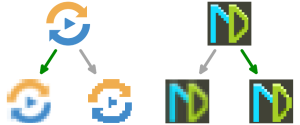
\includegraphics[width=0.5\linewidth]{imscaling.png}
  \caption{Image Scaling}
  \label{fig:imscaling}
  \end{center}
\end{figure}

We chose to implement the image downsizing in the following substeps:
\begin{enumerate}
\item \# Rows in image < 500: Size down to 50\%
\item 500 < \# Rows in image < 500: Size down to 33\%
\item 1000 < \# Rows in image: Size down to 25\%
\end{enumerate}

In order to compare the resulting Disparity Map to the Ground Truth, a upscaling after the Disparity Map computation is necessary. The algorithm used to upsample in our Code is called Nearest Neighbour Interpolation \cite{NNI} and is a very simple approach towards interpolation. Rather than calculate an average value by some weighting criteria or generate an intermediate value based on complicated rules, this method simply determines the nearest neighbouring pixel, and assumes the intensity value of it. This might result in a bad Peak Signal To Noise Ratio, but will definitely decrease the computational complexity compared to other algorithms


\chapter{Implementation}
\section{Overview}
In the following the implementation we chose for our project will be explained in more detail. Chapter 2.2 explains how the rotation and translation is calculated from the stereo image pairs correspondences and the camera specific parameters. Chapter 2.3 is going to go into more detail with the implementation of our Block Matching algorithm. Chapter 2.4 will focus on the usability of our algorithm with the Graphical User Interface (GUI).
\section{Rotation \& Translation with Correspondences}
In order to extract matching points between stereo images, one needs first to determine the Harris Corners. In this context, Harris Corner Detection is an algorithm introduced by Chris Harris and Mike Stephens \cite{harris1988combined} in 1988 which is used to extract corners and edges from images.

The corners detected in the images has to be compared using Normalized Cross Correlation which compares two points and determines if they match or not. To improve and select the robust points one need to use RANSAC Algorithm \cite{cantzler1981random} which selects the matching points that have high rates. The description below resumes the stated process.

\begin{enumerate}
\item Convert image to Grayscale (if it is colored)
\item Calculate Harris features
\item Find correspondences \& filter for stable ones with RANSAC
\item Calculate essential matrix by using the camera parameters \& robust correspondences
\item Calculate Rotation \& Translation by using the essential matrix
\end{enumerate}

The resulting rotation \& translation show how the positon of the two cameras differs in 3D space and is one of the outputs of the \textit{challenge.m} function.

\section{Disparity Algorithm}
Sourcecode blockmatching: \cite{Chris} \\
source ncc / ssd / sad \cite{fouda2015normalize}
\section{Graphical User Interface}

\chapter{Results}

\begin{table}
\centering
\begin{tabular}{lllll}
	\hline
	\textbf{Bild} & \textbf{Image size} & \textbf{Parameter} & \textbf{PSNR} & \textbf{Time} \\
	\hline
	Motorcycle & 0 & 0 & 0 & 0 \\
	Playground & 0 & 0 & 0 & 0 \\
	Sword & 0 & 0 & 0 & 0 \\
	Terrace & 0 & 0 & 0 & 0 \\
	\hline
\end{tabular}
\caption{Results}
\label{tab:threecols}
\end{table}

\chapter{Conlusion}



% Das folgende LaTeX-Makro erzeugt aus der Datei diplomarbeit.bib das
% Literaturverzeichnis.
\bibliography{Group29_documentation}

\end{document}
